\documentclass[12pt,letterpaper]{report}
\usepackage[utf8]{inputenc}
\usepackage{fancyhdr}
\usepackage{multirow,tabularx}
\usepackage{pgfornament}
\usepackage[letterpaper,margin=1.3in]{geometry}
\usepackage{graphicx}
\usepackage[spanish]{babel}
\usepackage{listings}
\usepackage{tikz}
\usepackage{eso-pic}
\usetikzlibrary{positioning}
\newcommand{\nuevap}{\newpage \Marco}
\newcommand{\espacio}{\vspace{1cm}}
\newcommand{\Espacio}{\vspace{1.5cm}}
\graphicspath{../../../../../}
\lstset{
  inputencoding=utf8,
  extendedchars=true,
  literate= {á}{{\'a}}1 {é}{{\'e}}1 {í}{{\'i}}1 {ó}{{\'o}}1 {ú}{{\'u}}1 {Á}{{\'a}}1 {É}{{\'e}}1 {Í}{{\'i}}1 {Ó}{{\'o}}1 {Ú}{{\'u}}1,
  tabsize=2,
  basicstyle=\footnotesize,
  language=C,
  breaklines=true,
}

\pagestyle{fancy}
\fancyhf{}
\renewcommand{\headrulewidth}{0pt}

\newcommand{\Marco}{
  \begin{tikzpicture}[remember picture,overlay]
    \node[anchor=north, yshift=-1cm] at (current page.north){
      \pgfornament[symmetry=h,width=50pt]{72}
      \pgfornament[width=4.4in]{89}
      \pgfornament[symmetry=h,symmetry=v,width=50pt]{72}
    };
    \node[xshift=1in,yshift=-1.5cm] (A) at (current page.north west){};
    \node[xshift=1in,yshift=1.5cm] (B) at (current page.south west){};
    \node[xshift=-1in,yshift=-1.5cm] (AA) at (current page.north east){};
    \node[xshift=-1in,yshift=1.5cm] (BB) at (current page.south east){};
    \pgfornamentline{A}{B}{5}{71};
    \pgfornamentline{AA}{BB}{5}{71};
    \node[anchor=south, yshift=1cm] at (current page.south){
      \pgfornament[width=50pt]{72}
      \pgfornament[symmetry=h,width=4.4in]{89}
      \pgfornament[symmetry=v,width=50pt]{72}
   };
  \end{tikzpicture}
}
\newcommand{\Portada}{
  \begin{tikzpicture}[remember picture,overlay]
    \node[xshift=1in,yshift=-1.5cm] (A) at (current page.north west){};
    \node[xshift=1in,yshift=1.5cm] (B) at (current page.south west){};
    \node[xshift=-1in,yshift=-1.5cm] (AA) at (current page.north east){};
    \node[xshift=-1in,yshift=1.5cm] (BB) at (current page.south east){};
    \pgfornamentline{A}{B}{8}{84};
    \pgfornamentline{AA}{BB}{8}{84};
    \pgfornamentline{A}{AA}{1}{89};
    \pgfornamentline{BB}{B}{1}{89};
  \end{tikzpicture}
  %__________________________________________% TEXTO!
}

\begin{document}
\Portada{  
  \begin{center}
    {\Large
    %\includegraphics[scale=0.8]{../../../../../escudo-linea-horizontal-png.png}\\
    \espacio
    División de Inenierías Campus Irapuato Salamanca \\
    Universidad de Guanajuato
    \espacio
    Clase: Inteligencia artificial\\
    \espacio
    Profesor: Dr. Carlos Hugo García Capulín\\
    Estudiante: Brandon Marquez Salazar\\
    \espacio
    \espacio
    Tarea 1\\
    \espacio
    \espacio
    Uso de PSO Velocity Clamping\\
    \espacio
    \espacio
     Entrega 25 de Abril del 2023
   }
  \end{center}
  }

  \nuevap
  \large
  \section*{Introducción}
  La
  La optimización de enjambre de partículas (PSO) se considera importante en la inteligencia basada en enjambre.
  El PSO está relacionado con el estudio de los enjambres; donde se trata de una simulación de bandadas de pájaros.
  Se puede utilizar para resolver una amplia variedad de problemas de optimización. Es un método heurístico el cual,
  esencialmente, busca la solución a un modelo, basado en elementos específicos y un conjunto de estructuras, que
  emulan el comportamiento de un conjunto de individuos quienes buscan una posición espefífica, que se evalúa según
  el modelo planteado.
  \section*{Planteamiento del problema}
  El problema que se nos plantea, es la búsqueda del valor más alto, utilizando el método de PSO con truncamiento de
  velocidad, d'a siguiente ecuación:\\ \\
  \begin{math}
    {\centering
      y(x,y)=\left( \frac{-((x+1)^2+(y-3.14)^2)}{5^2} \right)+\cos(2x)+\sin(2y) 
    }
  \end{math}
  \section*{Descripción del programa}
  El programa consta de una estructura PARTICULA y una estructura ENJAMBRE. La estructura partícula tiene los valores
  importantes de posición y evaluación respecto al modelo matemático. También, se tienen funciones que permiten la
  operación d'os elementos del enjambre, su inicialización, actualización e interacción.
  El código está dividido en una cabecera que define las operaciones esenciales del algoritmo, las estructuras y el
  prototipo de las dos funciones q'el usuario puede definir: función objetivo (el cual albergará al modelo
  matemático), función proceso (que albergará'l proceso que llevará, desde la creación del enjambre, las evaluaciones,
  entre otros elementos del procesamiento, hasta su limpieza).
  \section*{Código utilizado}
  \subsection*{Cabecera}
  \lstinputlisting[language=C++]{../../pso.h}
  \subsection*{Definiciones}
  \lstinputlisting[language=C++]{../../pso.c}
  \subsection*{Programa principal, definición de modelo y proceso pso}
  \lstinputlisting[language=C++]{../VelClamp.c}
  \section*{Pruebas y resultados}
  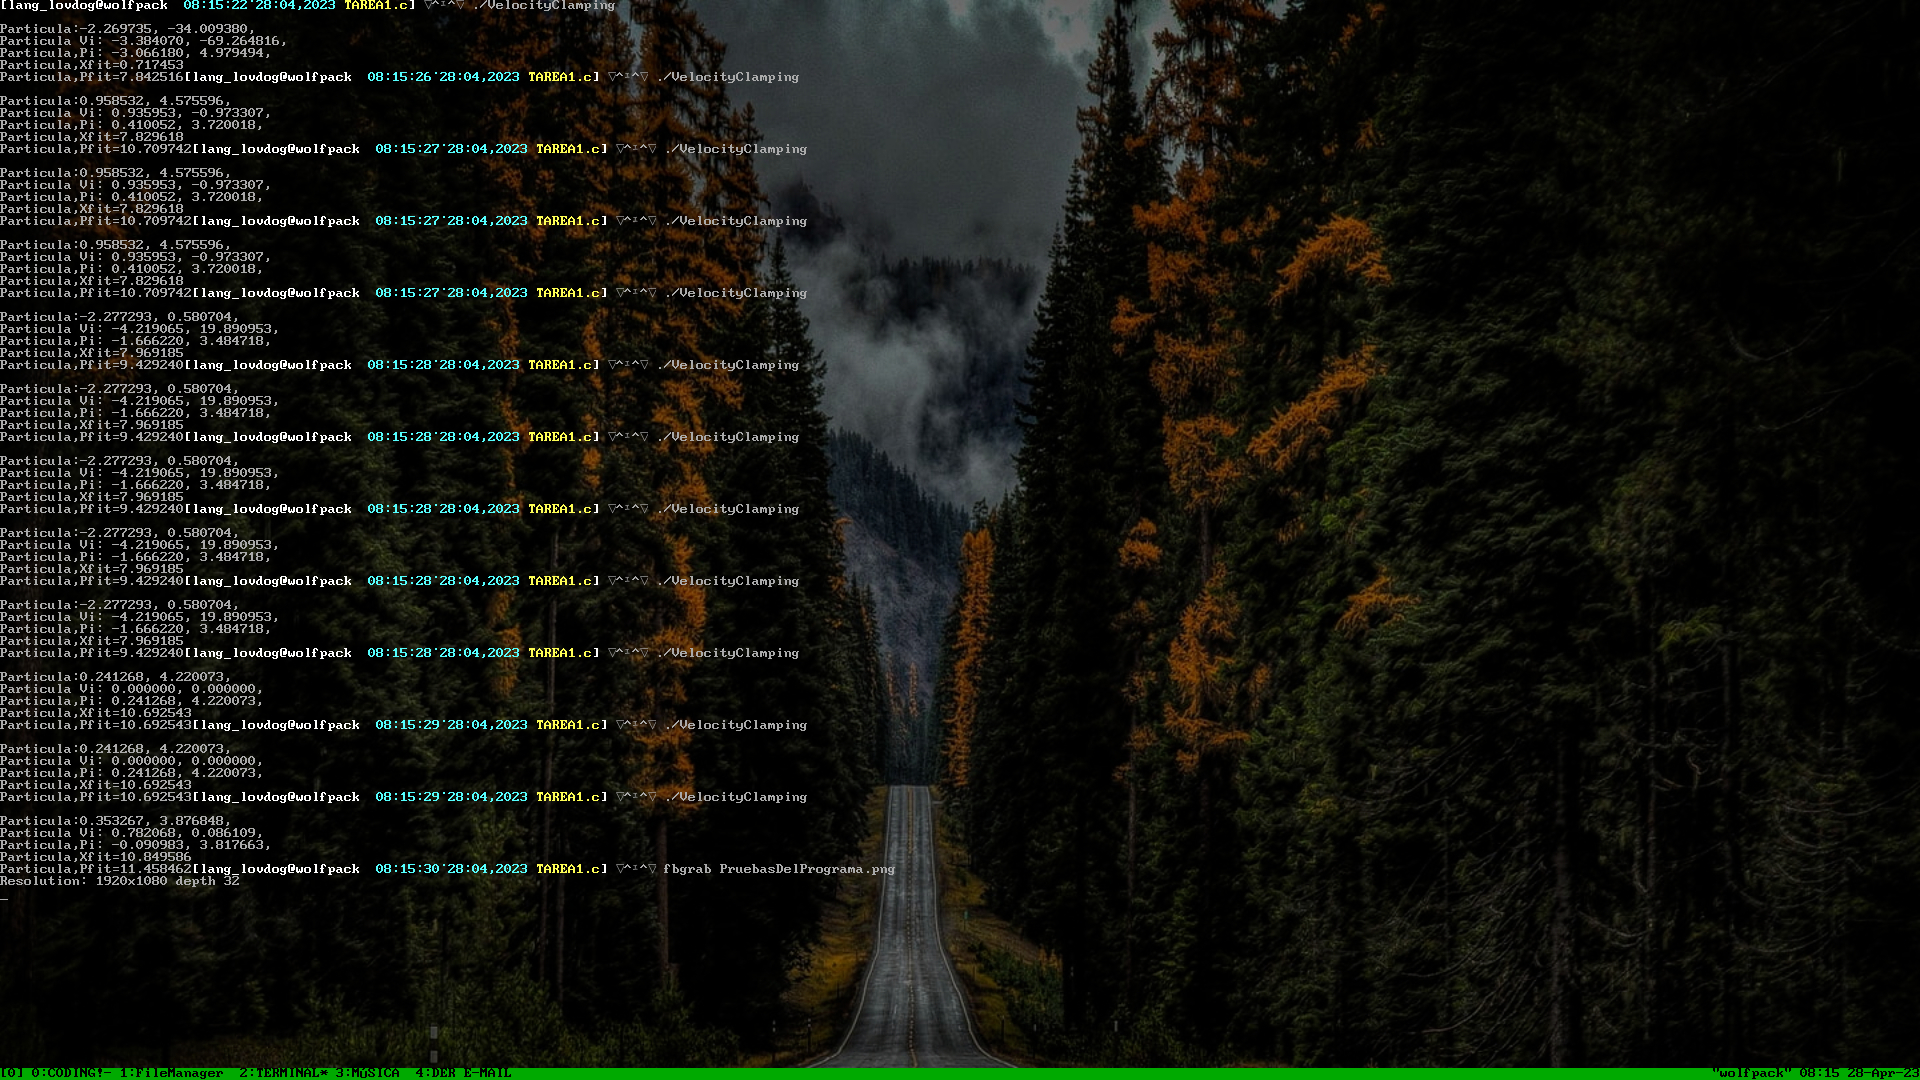
\includegraphics[scale=0.45,trim= 0 7cm 38cm 0,clip]{../PruebasDelPrograma}
  \section*{Conclusión}
  Se puede percibir la forma en que el método de partículas, dentro de la simplesa de su planteamiento matemático
  y de la compejidad de su composición, permite un procesaamiento de esencialmentos, preveyendo d'elementos
  estocásticos, los cuales permiten la generación de resultados en un amplio número de problemas; este método
  exige smiplesa en el modelo matemático que se desea evaluar para evitar una carga fuerte en el procesador, debido
  al número de evaluaciones que se realizan durante cada iteración según el número de partículas disparadas.
\end{document}
